\documentclass{beamer}

\usetheme{Madrid}
\usecolortheme{seagull}
%\usepackage{fancyhdr}
%\usepackage{titling}
%\pagestyle{fancy}
%\pagenumbering{gobble}
%\fancyhead[L]{Math 572}
%\fancyhead[C]{Final Project Report}
%\fancyhead[R]{Alex Shulhan}
%\fancyfoot[L]{Fall 2026} %% title
%\fancyfoot[R]{\thepage} %% page number
%\fancyfoot[C]{} %% center
%\setlength{\headheight}{25pt}
%\renewcommand{\footrulewidth}{0.4pt}
%\setlength{\footheight}{50pt}
%%%%%%%%
%\usepackage{fullpage}
\usepackage{amsmath, amsfonts, amscd, epsfig, amssymb, amsthm}

%\newcounter{chapter}
%\numberwithin{section}{chapter}
\theoremstyle{definition}
\newtheorem{exercise}{Exercise}
%\newenvironment{solution}
%{\begin{trivlist}\item[\bfseries Solution:]}
%{\end{trivlist}}
%\newcommand{\newproblem}[2]{
%\setcounter{exercise}{#1}\addtocounter{exercise}{
%	-1}\begin{exercise}#2\end{exercise}
%	}
\newcommand{\setcontext}[2]{\setcounter{chapter}{#1}\setcounter{section}{#2}}
\newcommand{\s}[1]{\mathcal{#1}}
\newcommand{\R}{\mathbb{R}}
\newcommand{\N}{\mathbb{N}}
\newcommand{\F}{\mathbb{F}}
\newcommand{\Z}{\mathbb{Z}}
\newcommand{\C} {\mathbb{C}}
\newcommand{\cov}{\text{Cov}}
\newcommand{\al}{\alpha}
\newcommand{\het}{\theta}
\newcommand{\h}{\hat}
\newcommand{\la}{\lambda}
\newcommand{\be}{\beta}
\newcommand{\hth}{\hat{\theta}}
\newcommand{\rc}{\mathscr{R}}
\newcommand{\n}{\mathscr{\nu}}
\newcommand{\e}{\mathbb{E}}
\newcommand{\si}{\sigma}
\newcommand{\Si}{\Sigma}
\newcommand{\ch}{\chi} 
%\newcommand{\exp}{\text{exp}}
%\newcommand{\labelenumi}{{\alph{enumi}}}

%\title{Practicing}
%\author{Name}
%\maketitle




\usepackage{graphicx}
\usepackage{listings}
\usepackage{hyperref}
\usepackage{xcolor}
\usepackage{subfig}
\usepackage{mwe}
\usepackage[style=authoryear, backend=bibtex]{biblatex}
\addbibresource{references.bib}
\definecolor{matlabblue}{RGB}{0, 91, 150}
\definecolor{matlabgray}{RGB}{240, 240, 240}

\lstdefinestyle{matlab}{
    language=octave,
    backgroundcolor=\color{matlabblue},
    basicstyle=\ttfamily\scriptsize,
    keywordstyle=\color{matlabgrey}\bfseries,
    commentstyle=\itshape\color{gray},
    showstringspaces=false,
    frame=single,
    numbers=left,
    numberstyle=\tiny,
    tabsize=2
}

\setbeamertemplate{frame footer}{}
\AtBeginSection[]{
  \begin{frame}[c, noframenumbering]
    \sectionpage
  \end{frame}
}
%\usepackage{bibtex} % biblatex
%\addbibresource{references.bib} % reference file
% \usepackage{unicode-math}
% \setmainfont{sTIX Two Text}
% \setmathfont{sTIX Two Math}

\title{Mutual Fear Model}
\subtitle{MATH 572}
\author{Alexander Shulhan}
\begin{document}
\maketitle
\section[allowframebreaks]{Background and Tools}
\begin{frame}
  \begin{columns}[c]
    \begin{column}{0.4\textwidth}
  \begin{figure}
    
\includegraphics[height=0.9\textheight,width=0.5\textwidth,keepaspectratio]{Screenshot 2026-11-17 at 14-41-27 ProQuest Ebook Central - Reader.png}
    \centering
    \caption{Cover of Biography \footcite{gleditsch2020richardson}}
  \end{figure}
\end{column}
\begin{column}{0.5\textwidth}
  \begin{block}{Arms Race Dynamics}
  \begin{itemize}
    \item  Lewis Fry Richardson wrote a book on modelling war and peace, published posthumously \footfullcite{richardson1960arms}
    \item Nation's will react to one another's spending in an arms race.
    \item Their resources are limited in spite of constraints
  \end{itemize}
\end{block}
\end{column}
\end{columns}
\end{frame}
\begin{frame}{Questions}
  \begin{itemize}
    \item Under what conditions is peace reached? (stability)
    \item When will the spending escalate? (unstable)
    \item Can we use a phase angle $\phi$ to encapsulate system behaviour? (Ran out of time)
\end{itemize}
\end{frame}
\begin{frame}{Numerical Tools Used}
  \begin{itemize}
    \item \textbf{\href{https://octave.org/}{GNU Octave}:} free MATLAB, mostly cross compatible. Notable exception are \texttt{pplane8.m,pplane9.m,pplane2014b.m}$\dots$
      \begin{itemize}
	\item \texttt{ode45}: numerically solve the system
	\item \texttt{quiver,quiver3}: plot vector fields 
	\item \texttt{eig}: find the eigenvalues and eigenvectors for more general case. The undamped case was solved by hand analytically.
	\item \textbf{Codebase:} the current code for the project is on github \href{https://github.com/alexanderneva/math_572_project}{username: alexanderneva}.
      \end{itemize}
    \item \textbf{\href{https://gemini.google.com/app}{Gemini Thinking}:} questions about Richardson's book in absence of having a copy, help translating python to GNU Octave, GNU Octave questions like how to format plots and make labels, etc.
      \begin{itemize}
	\item \textbf{In particular: } How did Richardson view the relationships between 3 nations for grievance terms $\left[g_1,g_2,g_3\right]$. He explains it in the book \footcite{richardson1960arms} which is currently in the University's \href{https://www.ualberta.ca/en/facilities/f225-research--collection-resource-facility.html}{RCRF}.
      \end{itemize}
  \end{itemize}
\end{frame}
\section{Undamped Case}
\begin{frame}[allowframebreaks]{Undamped Analysis}
\begin{block}{Mutual Fear}
The initial value problem for the undamped model is given by
\begin{equation}\label{eq:model1}
  \begin{bmatrix}
    x^{\prime}\\
    y^{\prime}
  \end{bmatrix} = 
  \begin{bmatrix}
    0 & a \\
    b & 0 
    \end{bmatrix}
    \begin{bmatrix}
      x \\ 
      y
  \end{bmatrix},\quad x(0)=x_0,~y(0)=y_0,\quad a,b>0
\end{equation}
where $a$ and $b$ represent the spending per unit time of nations $A$ and $B$ respectively.
\end{block}
\begin{block}{Eigenvalues Determine Stability}
  The eigenvectors $v_1,v_2$ and eigenvalues $\lambda_1,\lambda_2$ of \autoref{eq:model1} are
\begin{equation*}
  \lambda_1,\lambda_2 = \pm \sqrt{ab},\quad P:=\left[v_1~v_2\right]=\begin{bmatrix}\sqrt{\frac{a}{a+b}} & \sqrt{\frac{a}{a+b}}\\
  \sqrt{\frac{b}{a+b}} & -\sqrt{\frac{b}{a+b}}
\end{bmatrix}
\end{equation*}
$\text{sign}(\lambda_1)\neq\text{sign}(\lambda_2)$ implies $p^\star$ is a saddle node.
\end{block}
\begin{block}{Analytical Solution}
\begin{equation}
  \psi(t) = c_1e^{\sqrt{ab}t}v_1 + c_2 e^{-\sqrt{ab}t}v_2,\quad c_1,c_2 \in \R
\end{equation}
\end{block}
\begin{figure}
  \centering 
  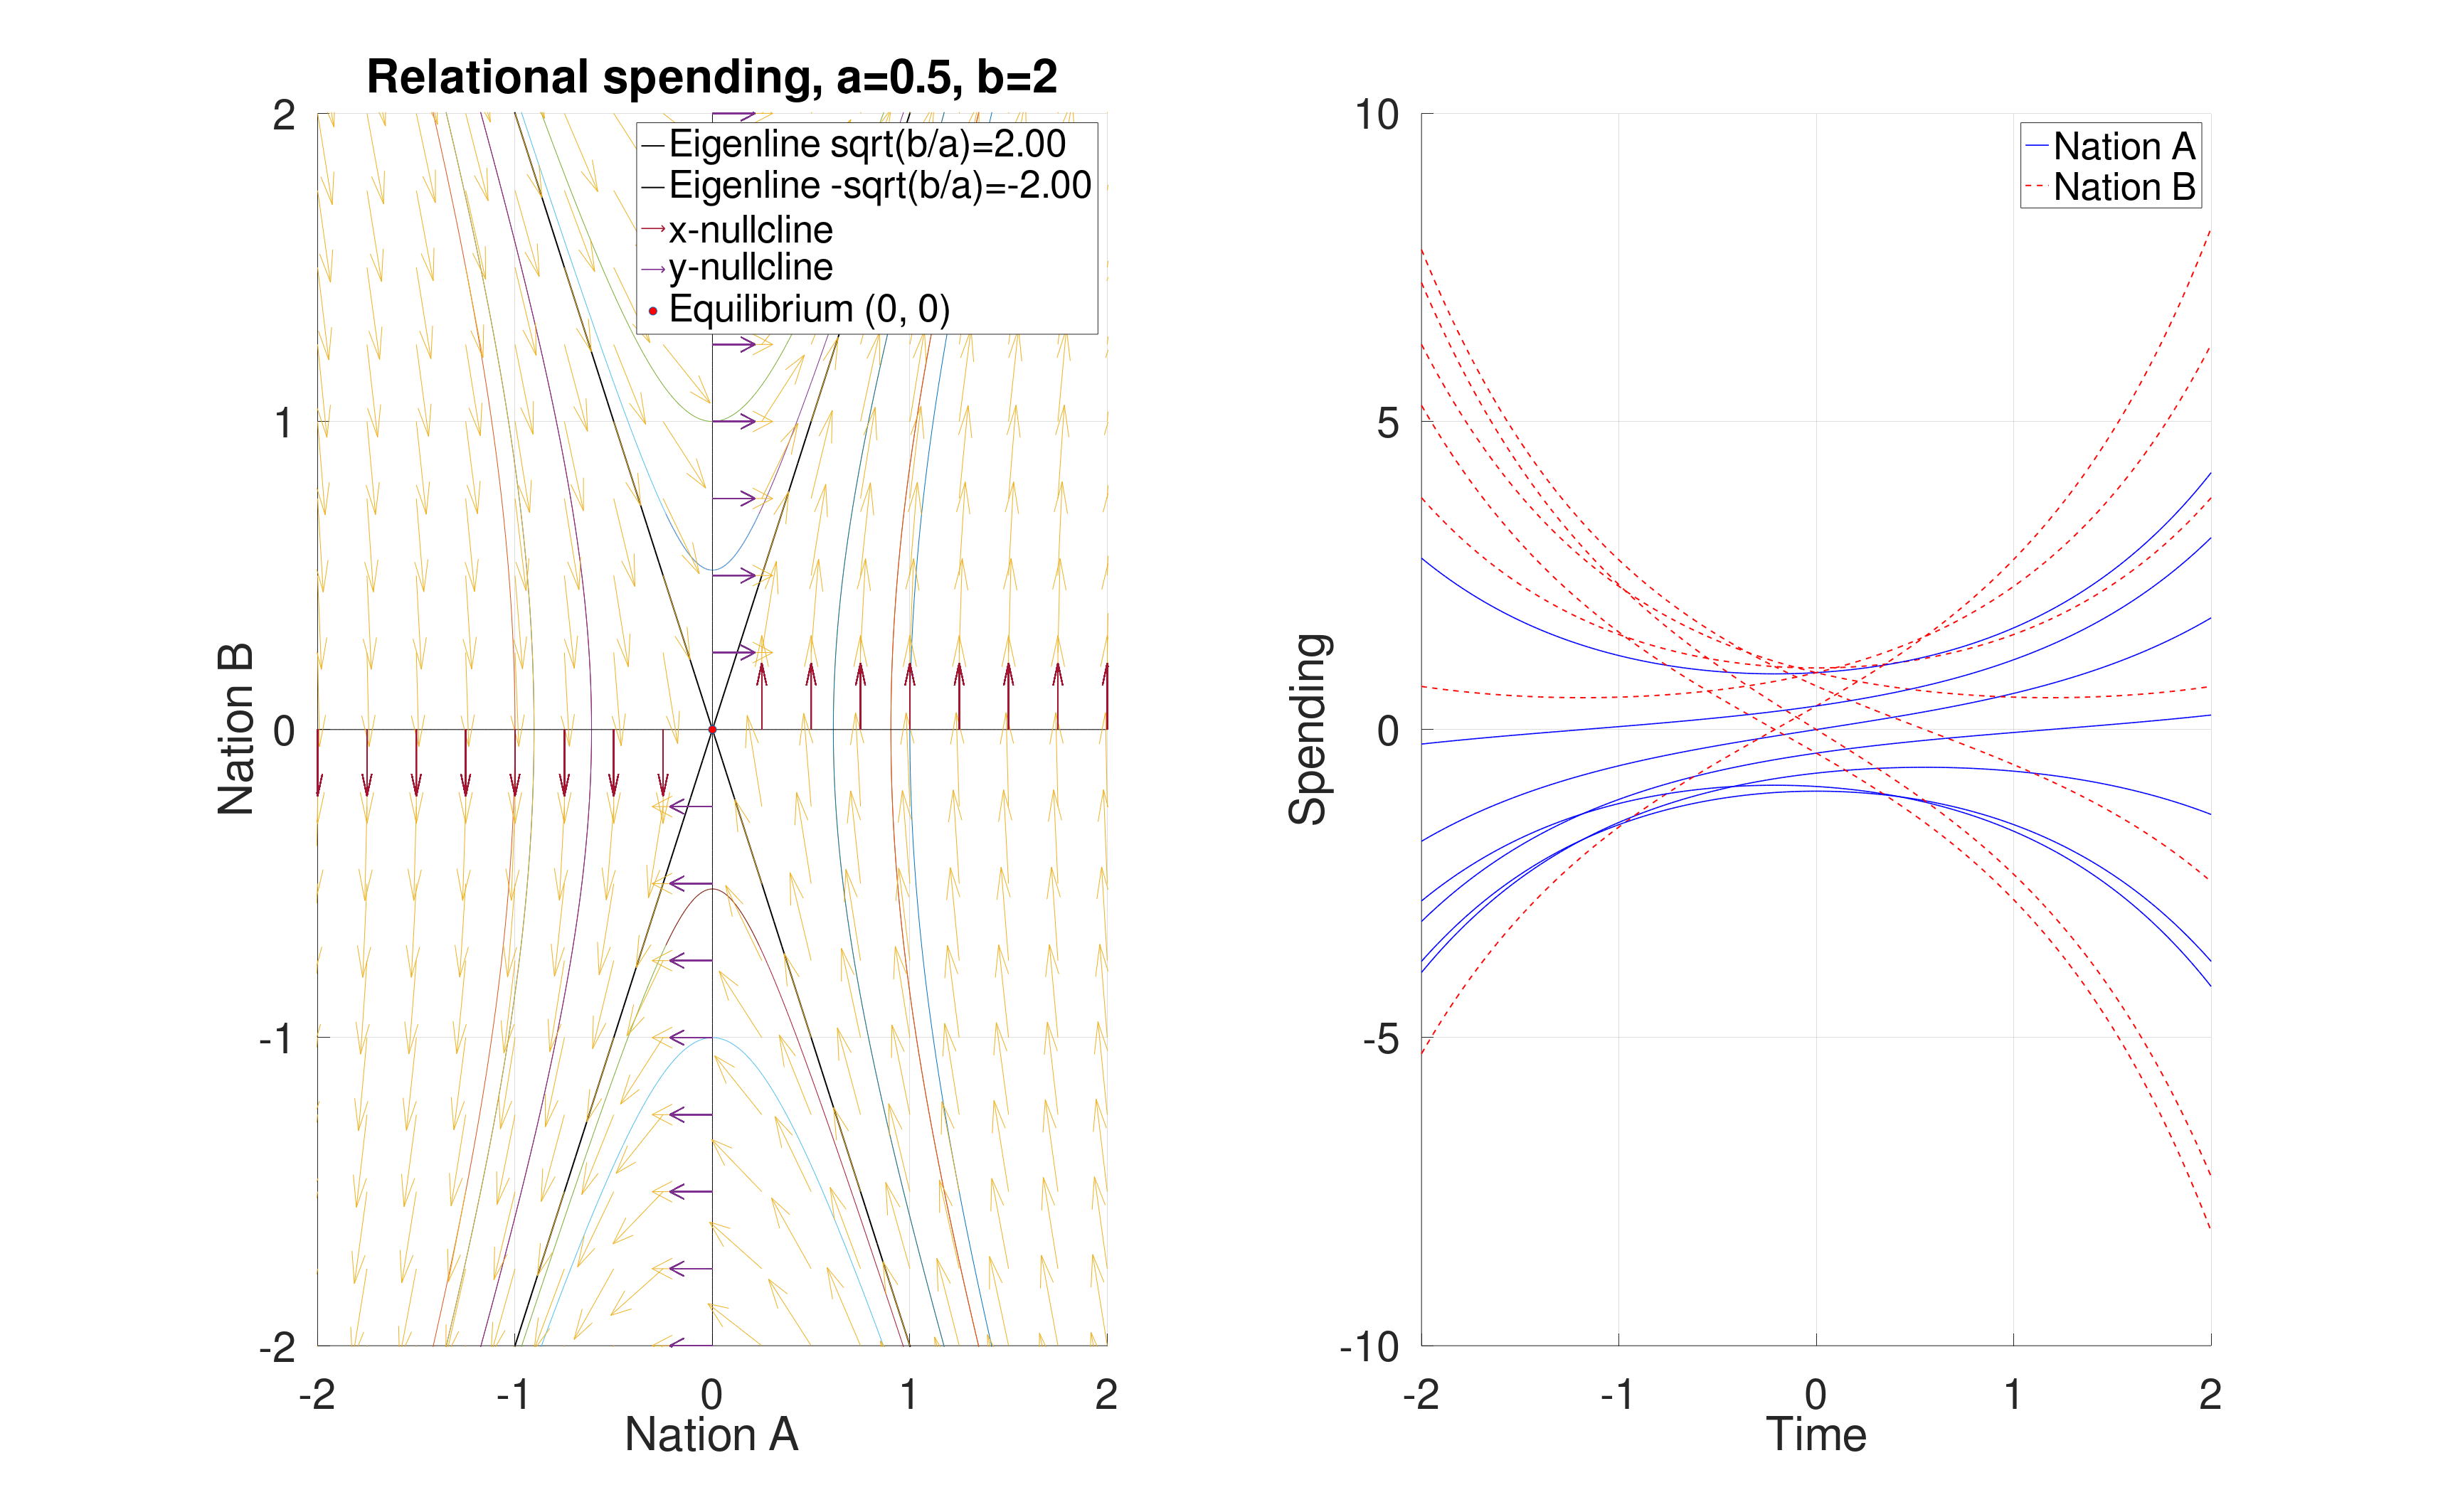
\includegraphics[height=0.9\textheight,width=\textwidth]{../figures/model_1_curves.png}
  \caption{Hyperbolae}
\end{figure}
\end{frame}
\section{2 Nations}
\begin{frame}[allowframebreaks]{Damped Case}\label{section2}
\begin{block}{Richardson}
The initial value problem for the Richardson model is given by
\begin{equation}\label{eq:richardson}
  \begin{bmatrix}
    x^{\prime}\\
    y^{\prime}
  \end{bmatrix} = 
  \begin{bmatrix}
    -m & a \\
    b & -n 
    \end{bmatrix}
    \begin{bmatrix}
      x \\ 
      y
      \end{bmatrix}+\begin{bmatrix}r \\ s\end{bmatrix},~x(0)=x_0,~y(0)=y_0,~a,b,m,n>0,r,s\in\R
\end{equation}
\end{block}
\begin{block}{Interpretation}
  \begin{itemize}
    \item \textbf{Economic dampening:} $m,n$ provide economic dampening in proportion to a nations own spending. These terms provide stability to the system since 
      \begin{equation}\label{eq:tr}\text{Tr }A = -m-n <0\end{equation}
    \item \textbf{Drift Term:} $r$ and $s$ determine how far the equilibrium $p^\star$ will be from $(0,0)$.
  \end{itemize}
\end{block}
\begin{block}{Routh-Hurwitz}
  Let \[A:=
  \begin{bmatrix}
    -m & a \\
    b & -n 
  \end{bmatrix}\]
  For characteristic polynomial $p(\lambda)$, recall the 2D Routh-Hurwitz conditions\footcite[Chap. 3]{MoghadasJaberiDouraki2019}. That is, $A$ defines a stable system if in
  \[
    p(\lambda)=\lambda^2-(\text{Tr }A)\lambda+\det{A}
  \]
  $\text{Tr }A < 0$ and $\det{A}>0$.
  Since the $\text{Tr }A<0$ (\autoref{eq:tr}), the character of our solutions can be seen from the determinant of our matrix $A$.
\end{block}
\end{frame}
\begin{frame}[allowframebreaks]{Equilibrium}
  Let $A$ denote the matrix from \autoref{eq:richardson} and $w:=\left[r,s\right]^T$. Assuming that $\det{A}\neq0$, we can find the equilibrium $p^\star=\left(x^\star,y^\star\right)$. By solving 
  \begin{block}{Finding the Equilibrium}
    \begin{align*}
      0&=Ap^\star+w\\
      \implies p^\star&=-A^{-1}w.
    \end{align*}
  \end{block}
  We can shift coordinates to center our system at the equilibrium by making the transformation
  \begin{block}{Coordinate Shift}
    \begin{equation}
      \tilde{v}=v-p^\star
    \end{equation}
  \end{block}
  We take the time derivative in the new coordinates
  \begin{block}{Substitution}
    \begin{align*}
      \tilde{v}^{\prime}=v^\prime
			&= Av+w\\
			&= A(\tilde{v}+p^\star)+w\\
			&= A\tilde{v}-AA^{-1}w+w\\
			&= A\tilde{v}
    \end{align*}
  \end{block}
  \begin{block}{Initial Conditions}
    \[
      \tilde{v}(0)= v(0)-p^\star
    \]
  \end{block}
\end{frame}
\begin{frame}{Animosity: $r,s>0$}
\begin{figure}
  \centering
  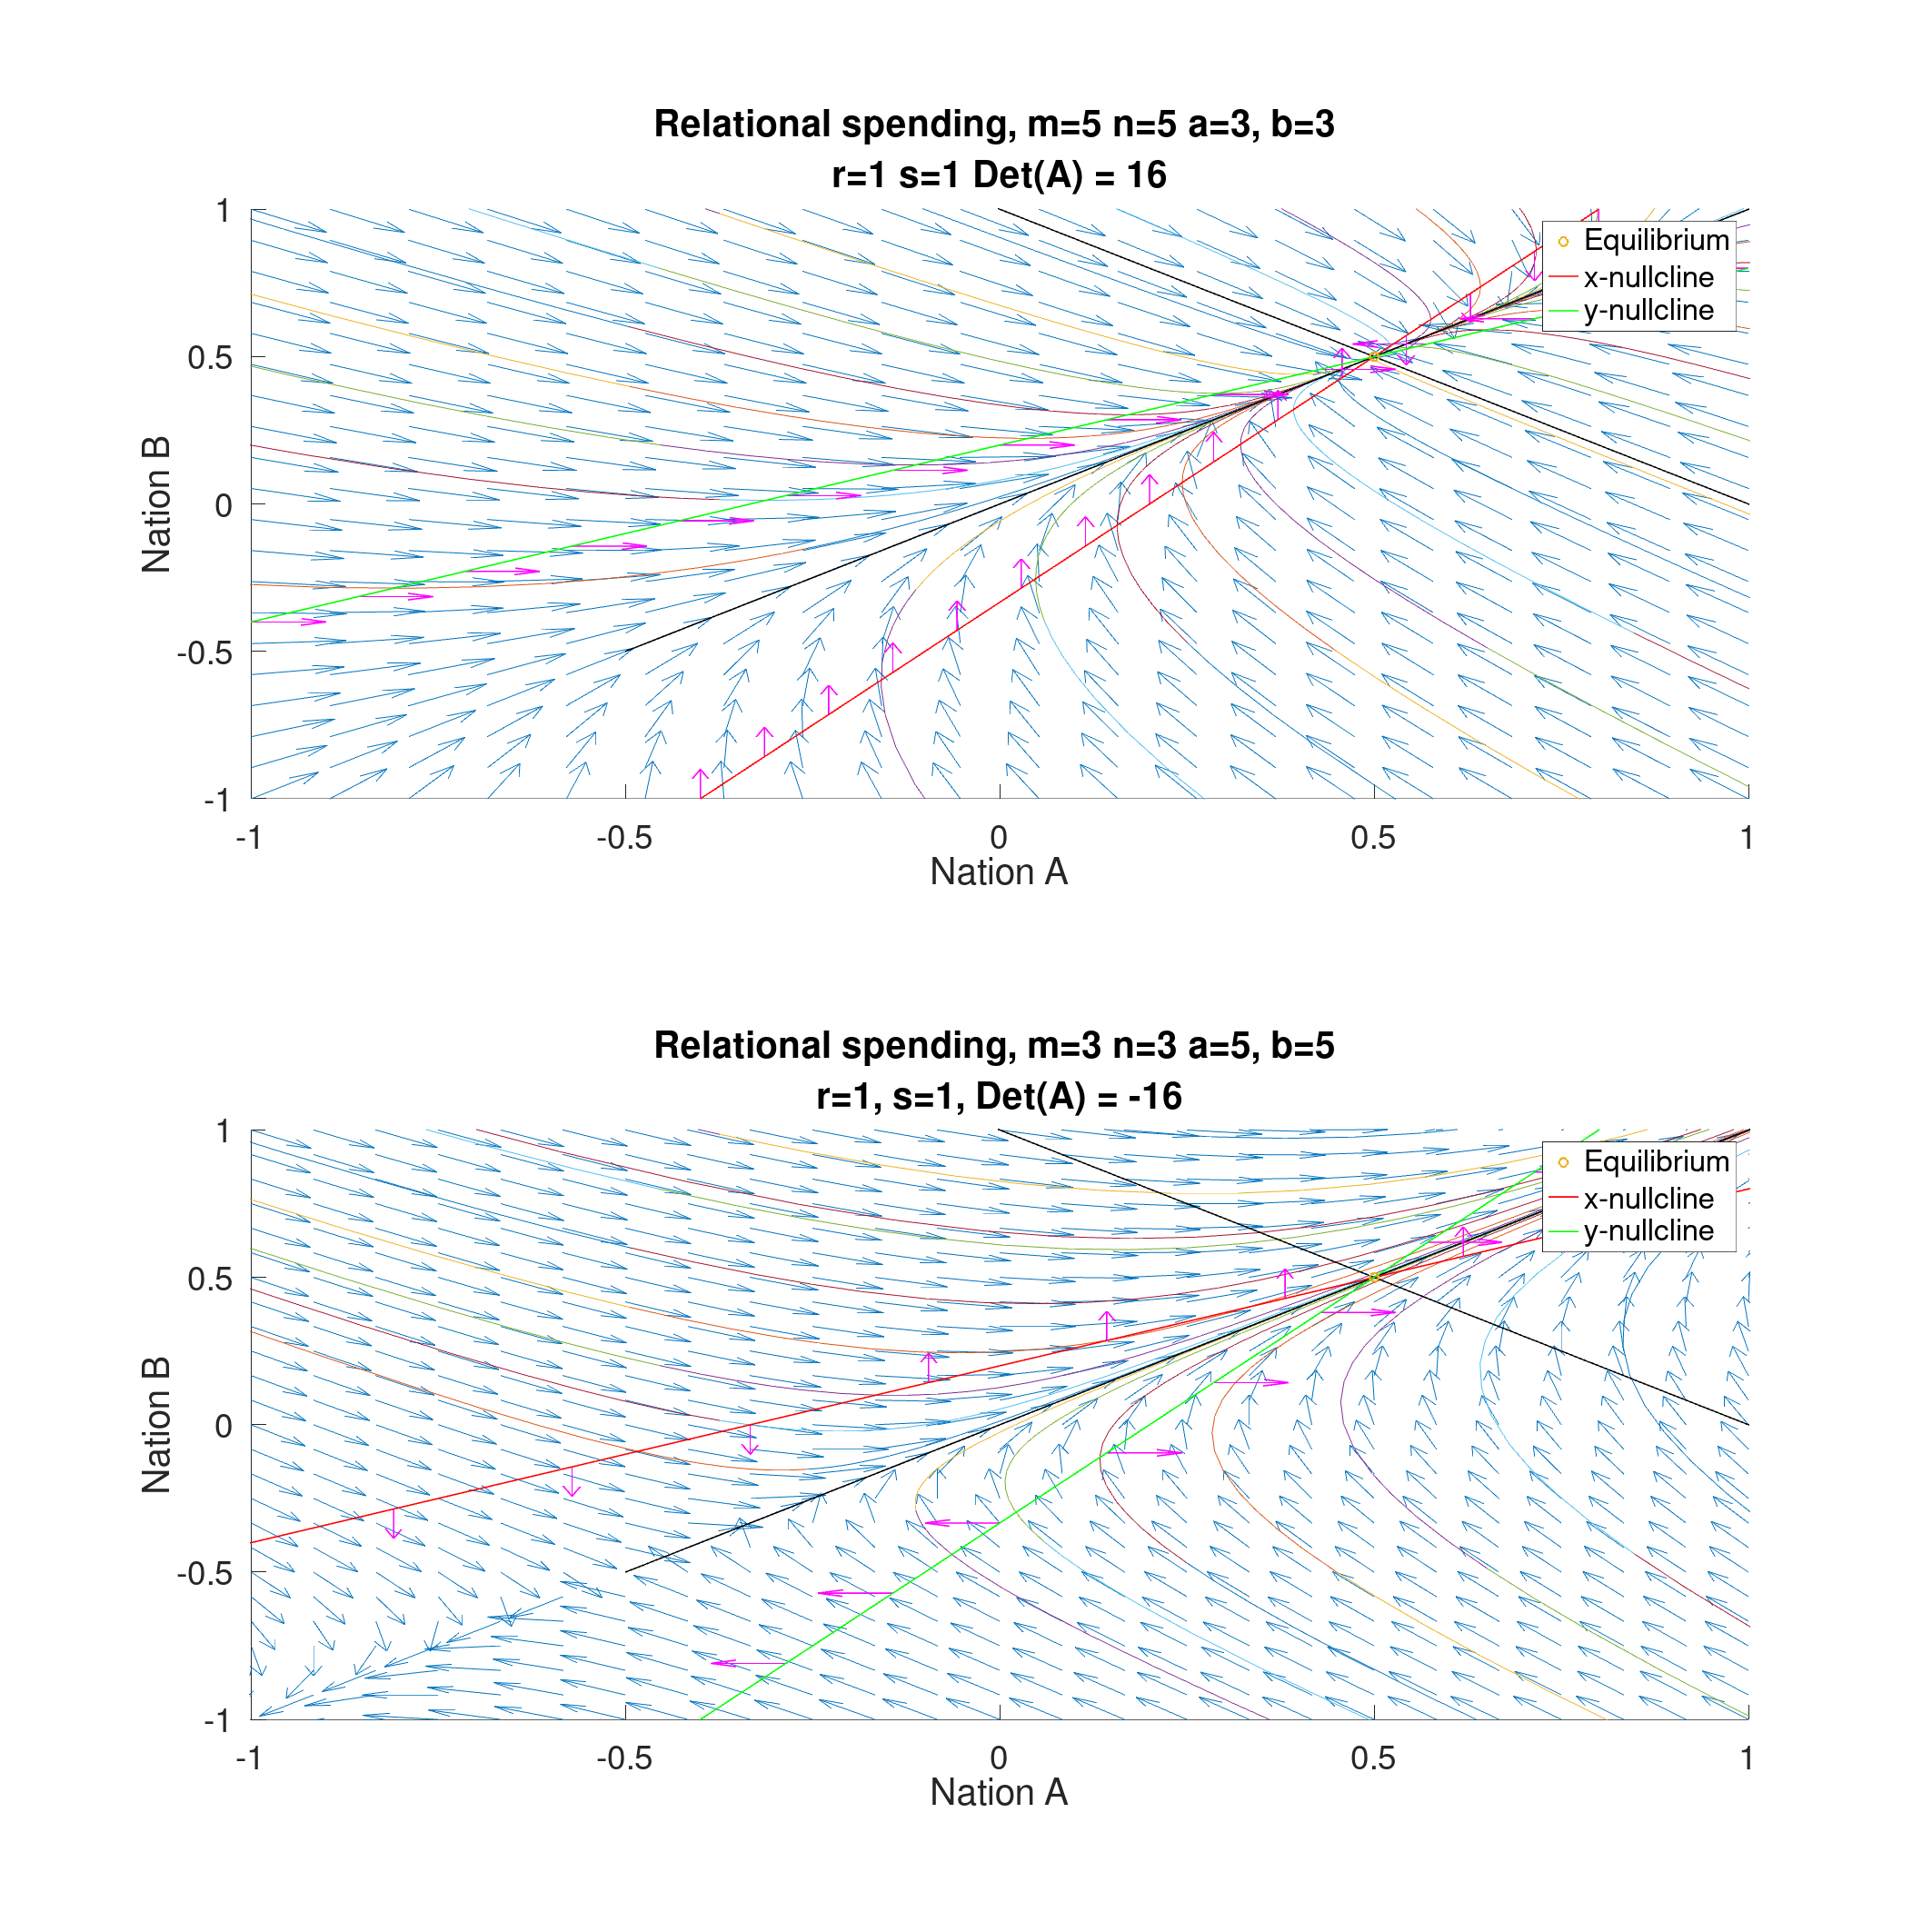
\includegraphics[height=0.9\textheight,width=\textwidth]{../figures/richardson_curves_1_1.png}
\end{figure}
\end{frame}
\begin{frame}{Nation B Good Will $r>0,s<0$}
\begin{figure}
  \centering
  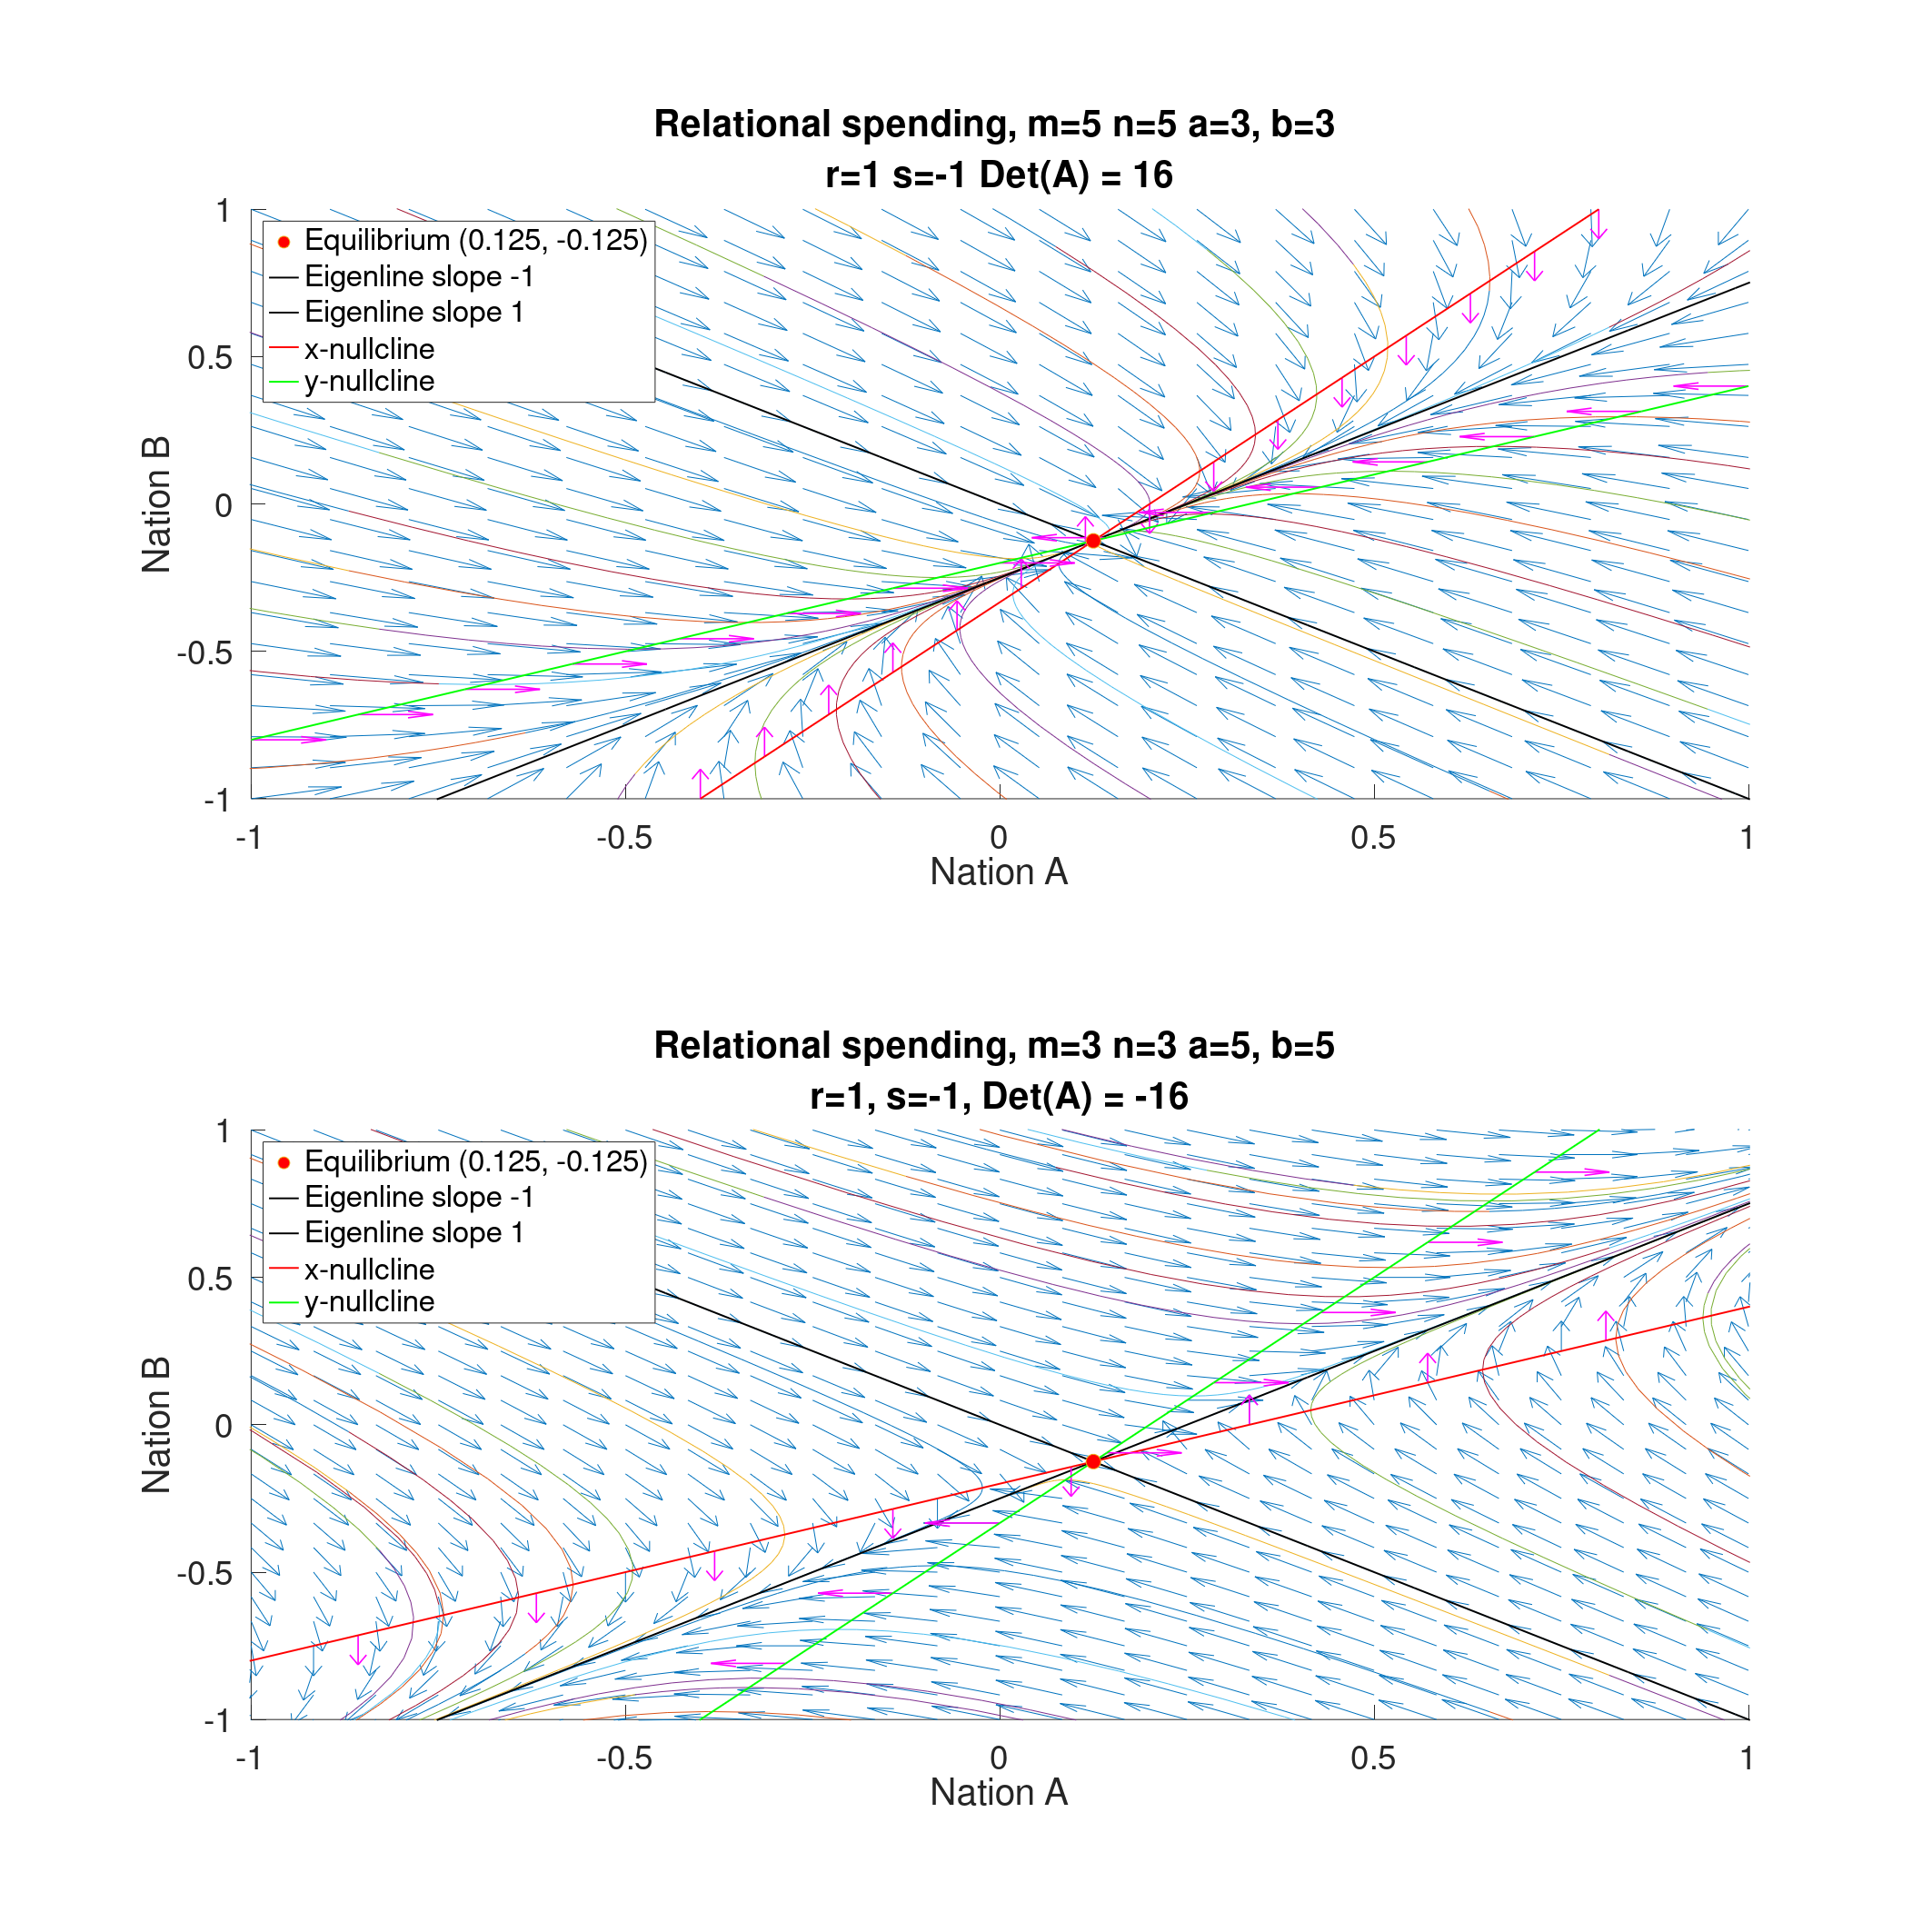
\includegraphics[height=0.9\textheight,width=\textwidth]{../figures/richardson_curves_1_-1.png}
\end{figure}
\end{frame}

\begin{frame}{Common Good Will $r,s<0$}
\begin{figure}
  \centering
  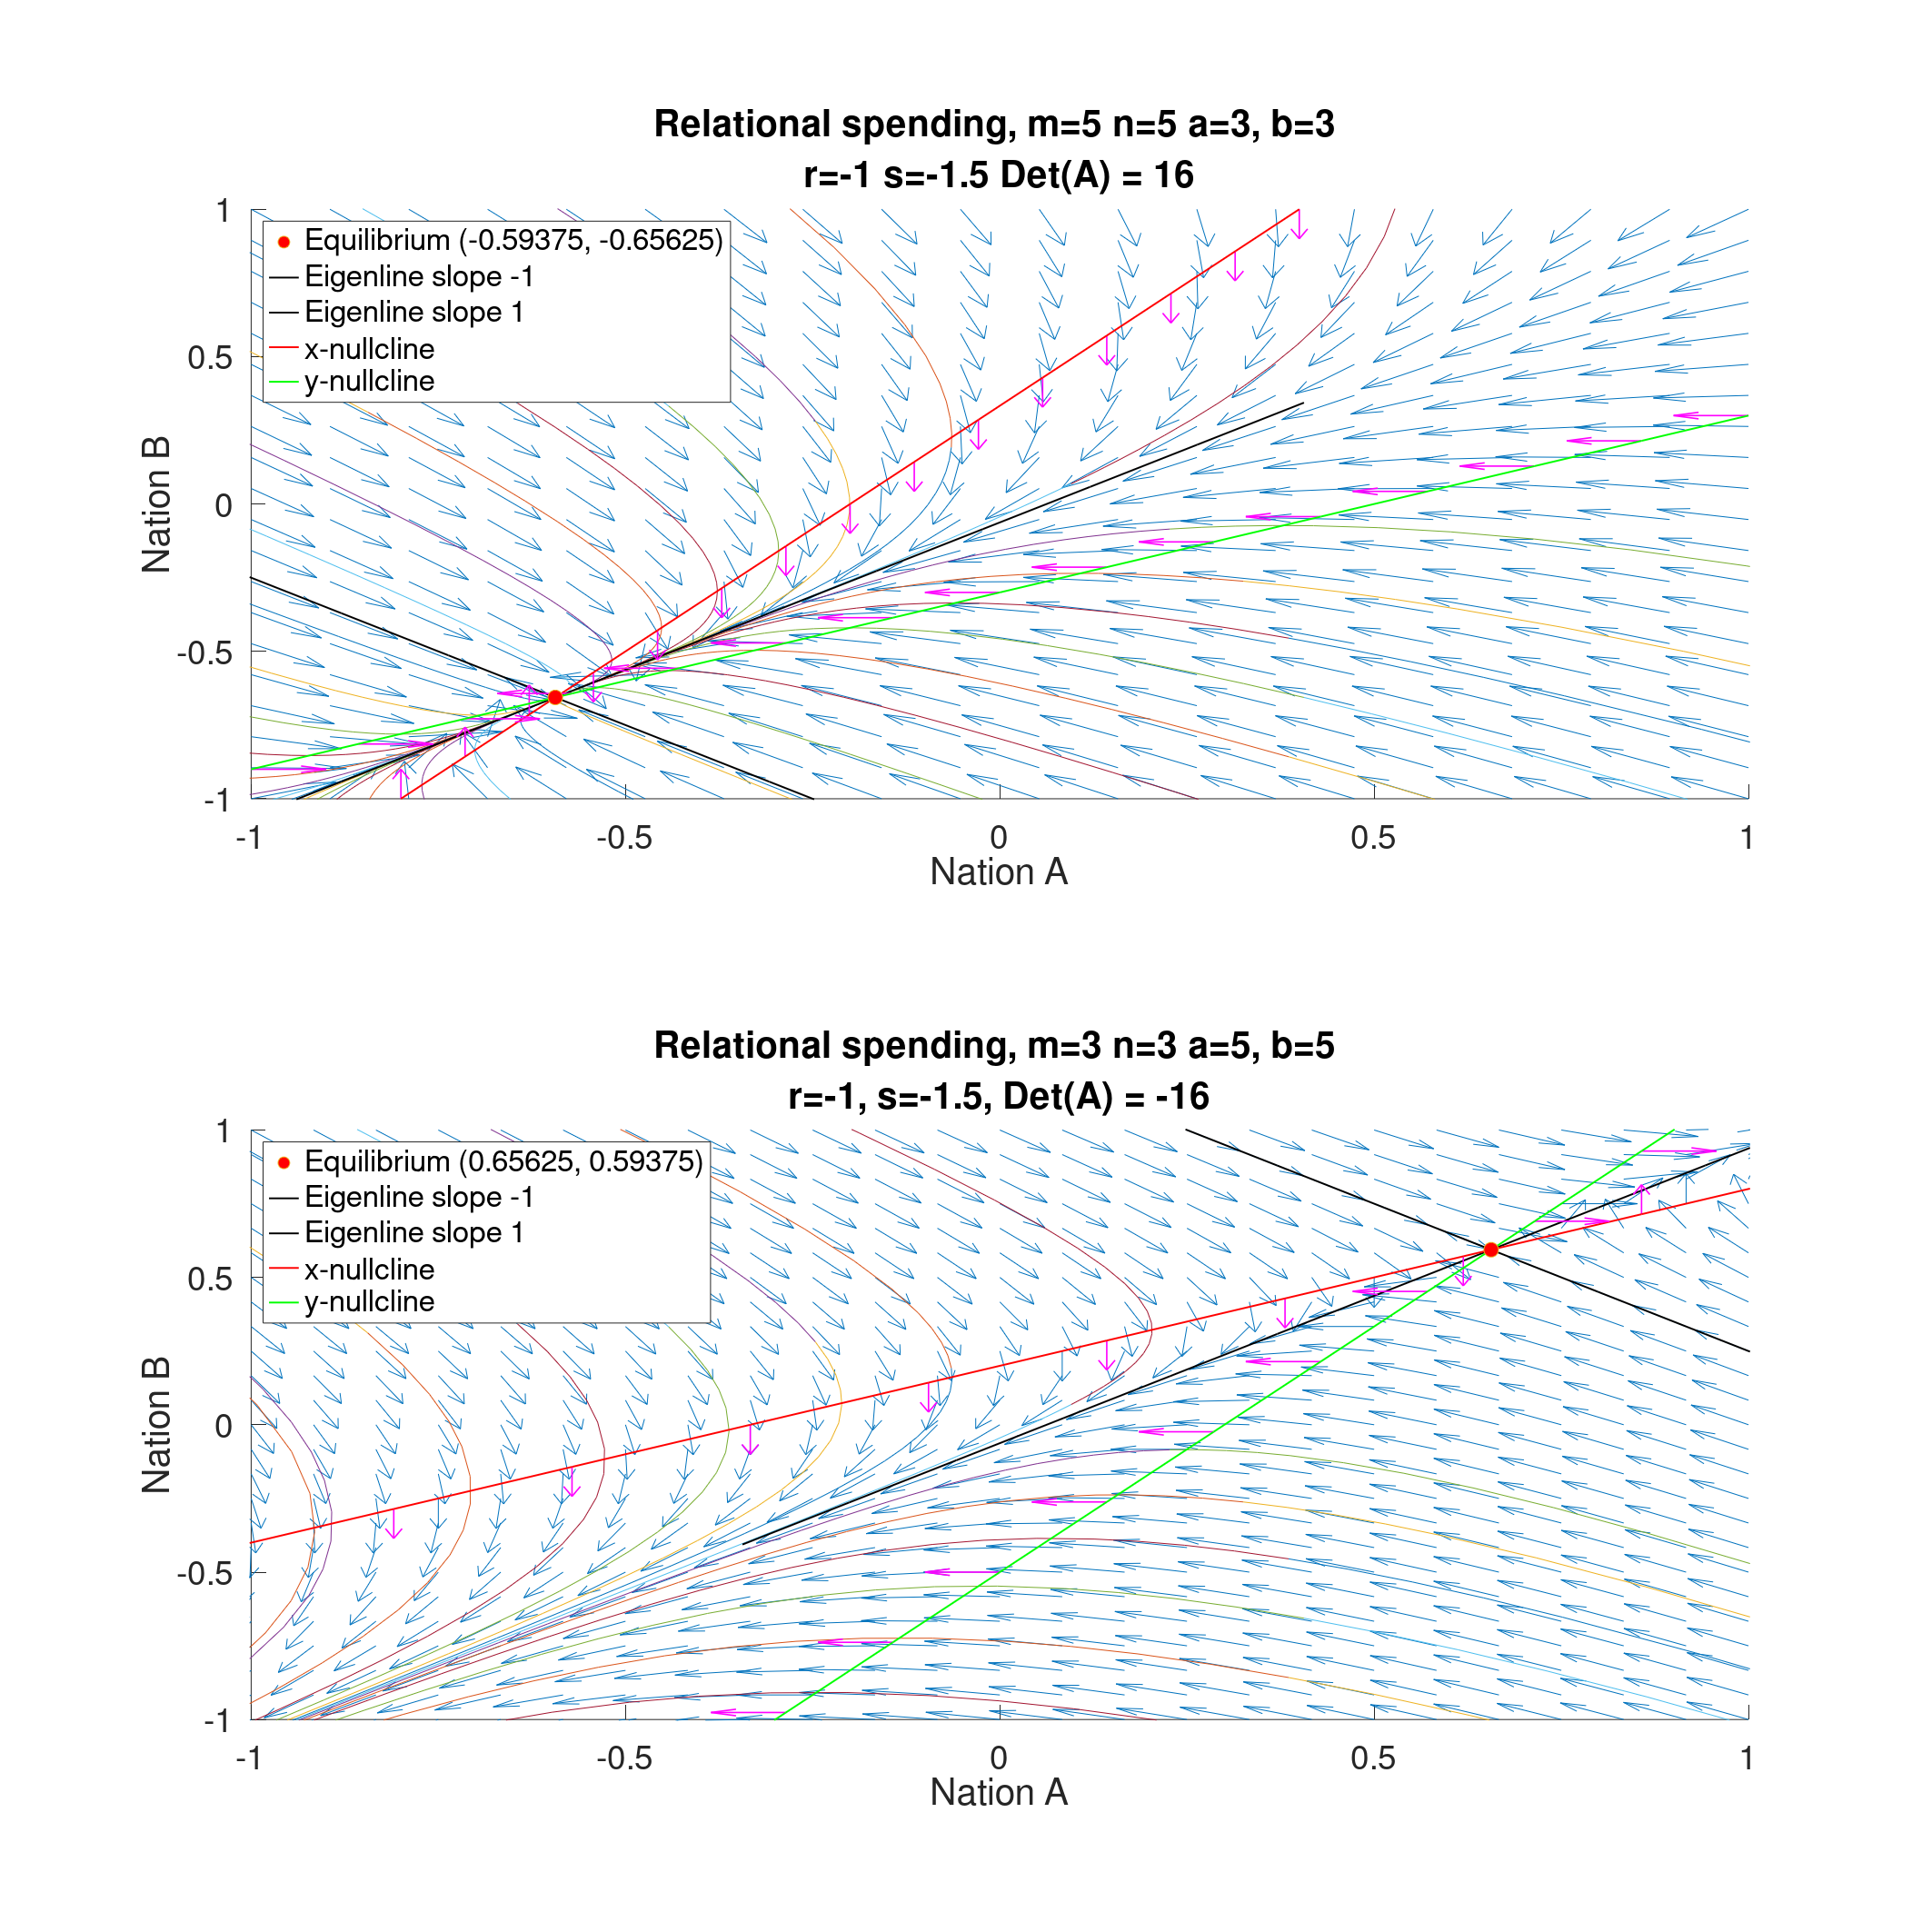
\includegraphics[height=0.9\textheight,width=\textwidth]{../figures/richardson_curves_-1_-1.5.png}
\end{figure}
\end{frame}

\begin{frame}{Observations}
  \begin{itemize}
    \item \textbf{Routh-Hurwitz} $det(A)>0$ shows stability 
    \item \textbf{nullclines} indicate direction changes of the vector field
    \item \textbf{Grievances:} inspite of good will, in the case that economic dampening does not outweigh spending $\det{A} <0$ positive feedback loop ensues. (Arms race)
\end{itemize}
\end{frame}
\section{3 Nations}
\begin{frame}
  \begin{block}{3 Nation Model}
    \begin{equation}\label{eq:nation}
    \begin{bmatrix}
      x^\prime \\ y^\prime \\ z^\prime
    \end{bmatrix}
    = \begin{bmatrix}
      -m & a & c_{13} \\
      b & -n & d_{23} \\
      c_{31} & d_{32} & -p
      \end{bmatrix}
      \begin{bmatrix}
	x \\ y \\ z
	\end{bmatrix}+\begin{bmatrix}g_{1}\\g_{2}\\g_{3}\end{bmatrix},\quad a,b,c_{31},c_{13},d_{32},d_{23},m,n,p>0
  \end{equation}
\end{block}
\begin{block}{Initial Conditions}
  \[ \begin{bmatrix}x(0)&y(0)&z(0)\end{bmatrix}^T=\begin{bmatrix}x_0 & y_0 & z_0\end{bmatrix}^T
\]
\end{block}
  \begin{block}{Variables}
    \begin{itemize}
      \item $m$,$n$,$a$,$b$ as in the previous model \autoref{eq:richardson}
      \item $c_{ij},d_{ij}$ spending rate of nation $i$ in response to spending of nation $j$
      \item $p$ economic decay of nation 3
      \item $g_i\in\R$ is the goodwill of nation $i$
    \end{itemize}
  \end{block}
\end{frame}
\begin{frame}[allowframebreaks]{Phase Plane Analysis}
  The coordinate transformation to $p^\star$ is of the same form as the 2D case. Thus, we can analyze the character of $A$, and employ the 3D Routh-Hurwitz criteria to judge the character of the solutions. The 3D Routh-Hurwitz conditions are\footfullcite{Li2018}
  \begin{equation}
    Tr{A}<0,\quad \det{A}<0,\quad\Lambda\text{Tr }A-\det{A} <0\\
  \end{equation}
  where $\Lambda$ is the sum of the principal minors of $A$
  \begin{equation}
    \Lambda =
  \end{equation}
  \begin{block}{Determinant}
    \begin{align*}
      \det{A}&= \begin{vmatrix}
      -m & a & c_{13} \\
      b & -n & d_{23} \\
      c_{31} & d_{32} & -p
    \end{vmatrix}\\
	     &= -m\begin{vmatrix}-n& d_{23}\\
	       d_{32} & -p\end{vmatrix}+n\begin{vmatrix}-m & c_{13}\\ c_{31} & -p\end{vmatrix}-p\begin{vmatrix}-m & a \\ b & -n\end{vmatrix}
    \end{align*}
  \end{block}
  \begin{itemize}
    \item Interpret the principal minors as relationship of nation $i$ with nation $j$, extending the analysis in \autoref{section2}
  \end{itemize}
\end{frame}
\begin{frame}{Richardson 3D}
  Since we are dealing with 12 parameters, we examine a couple of scenarios for the purposes of this presentation. First, let's define \emph{spending} power of a nation
    \begin{figure}
      \centering
      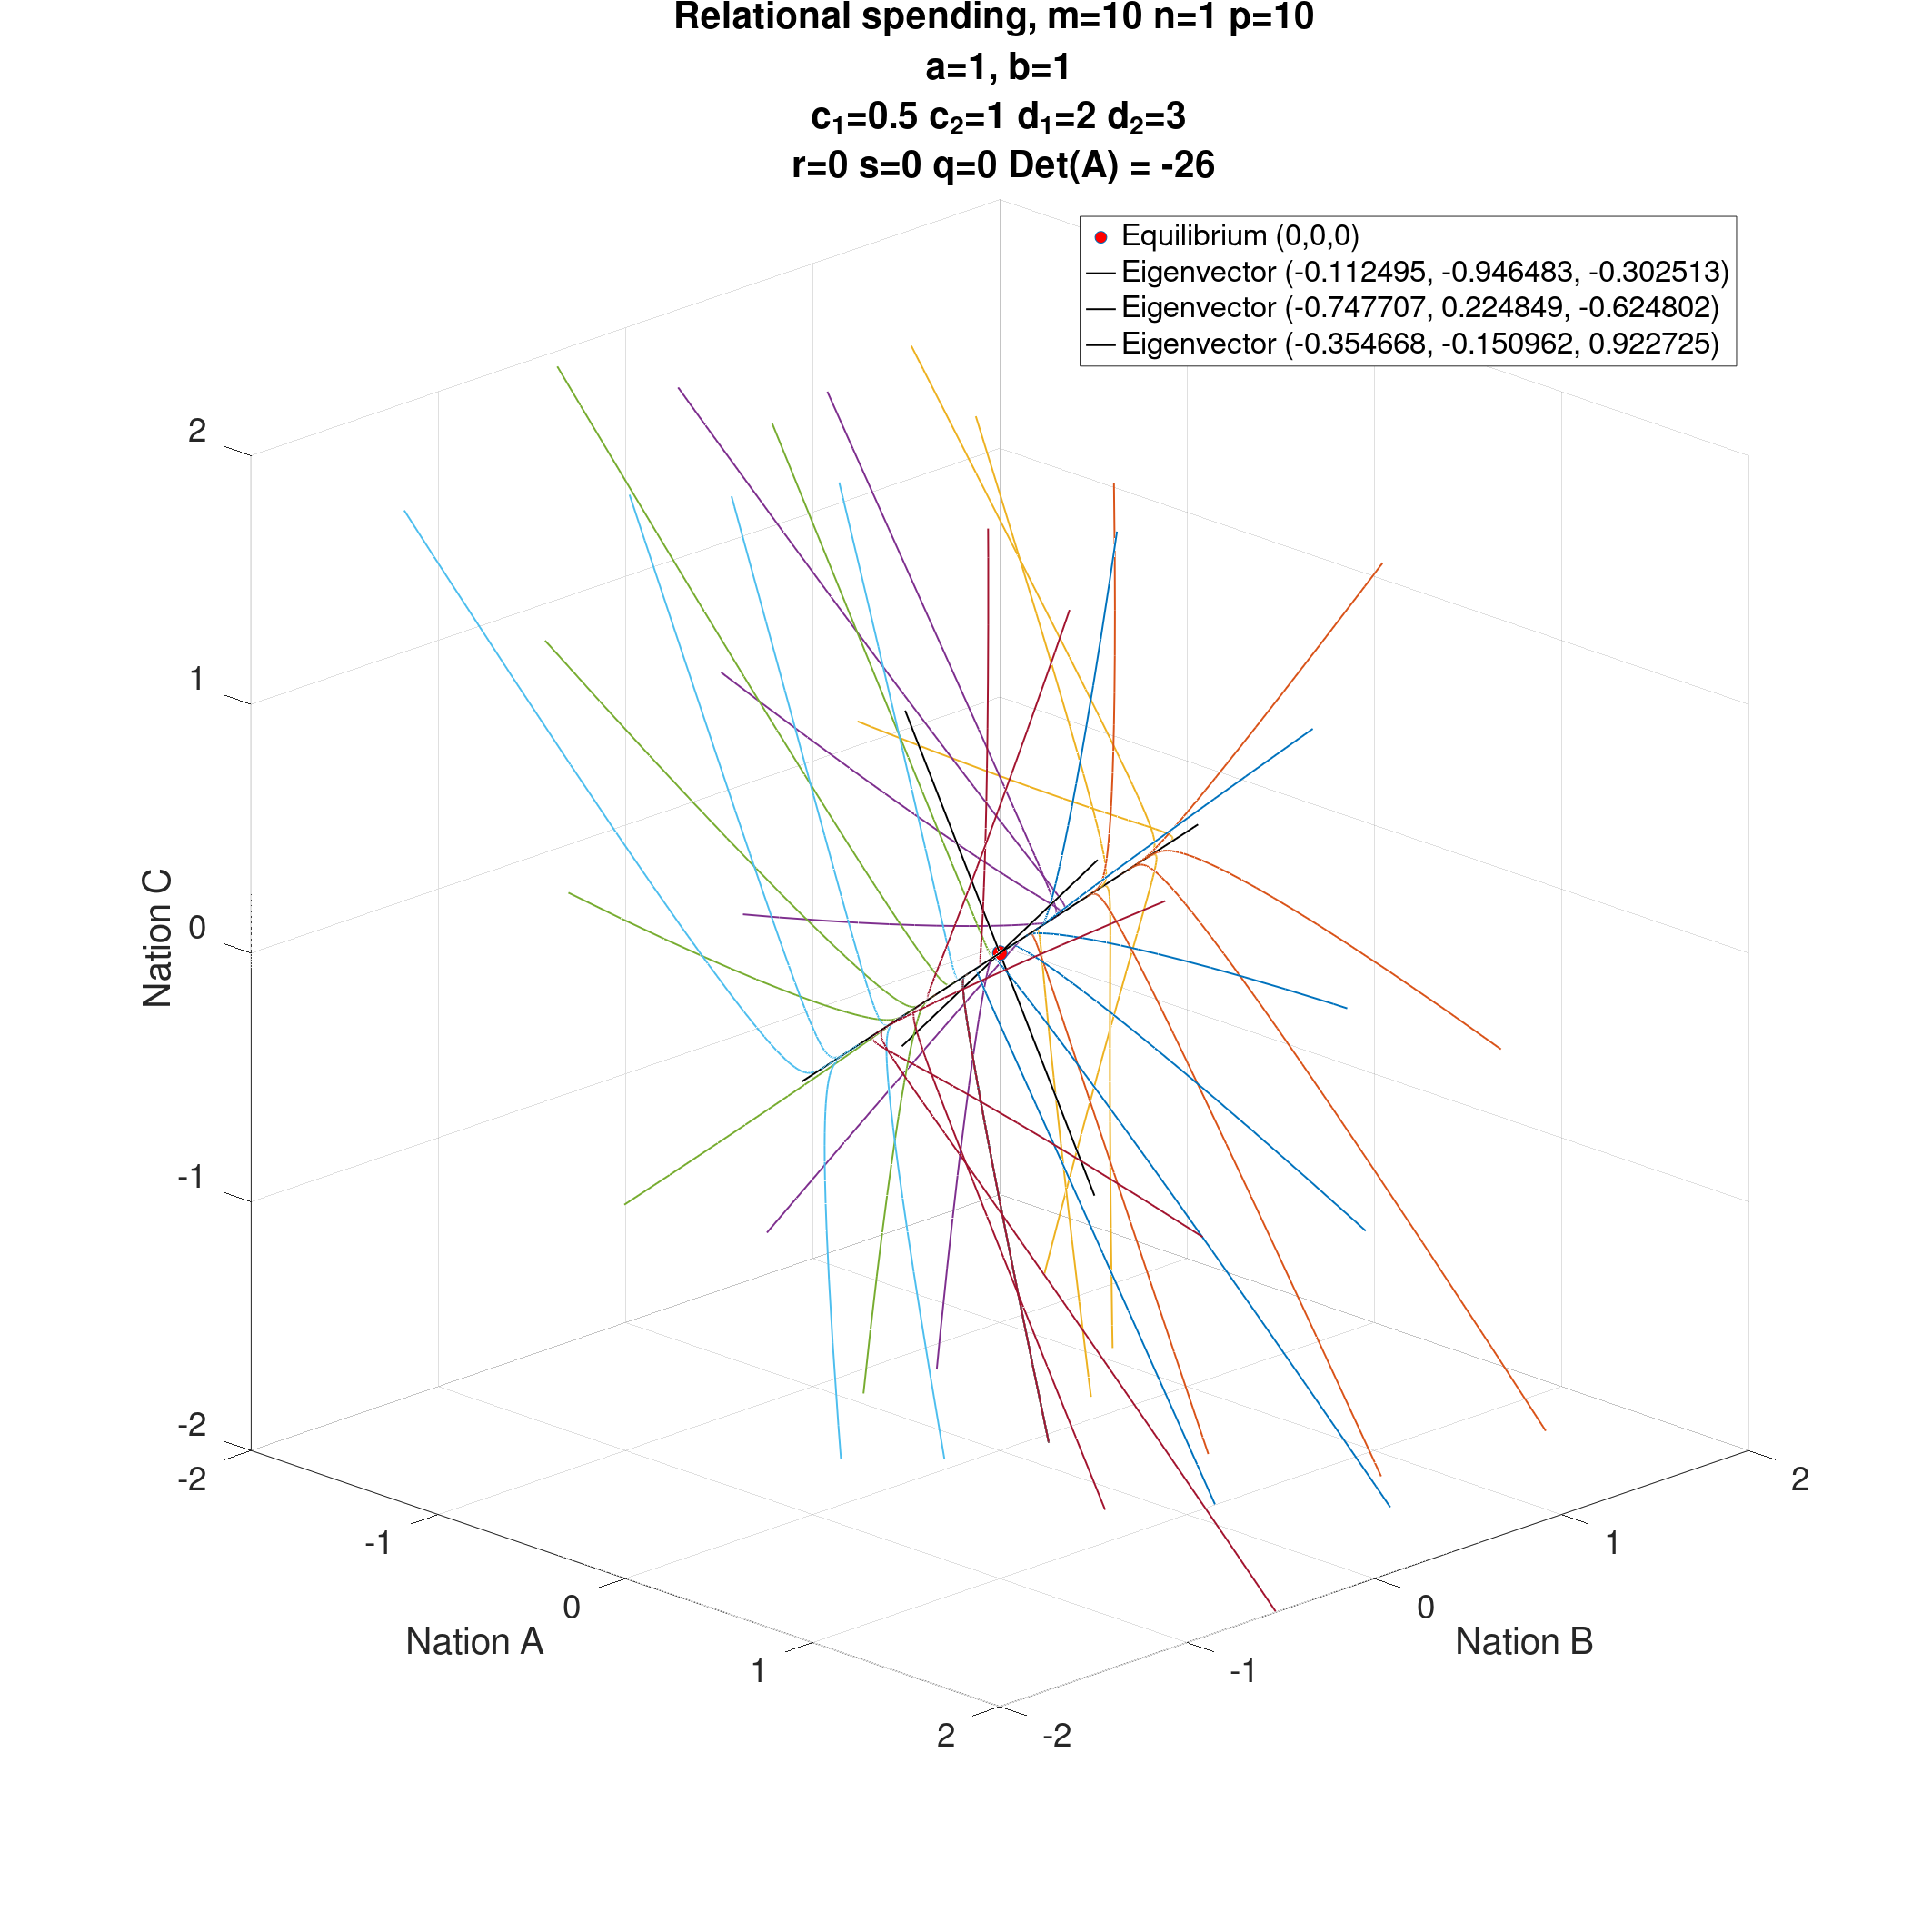
\includegraphics[height=0.9\textheight,width=\textwidth,keepaspectratio]{../figures/richardson_3D_0_0_0.png}
    \end{figure}
  \end{frame}
  \begin{frame}{Richardson 3D $r,q>0, s<0$}
    \begin{figure}
      \centering
      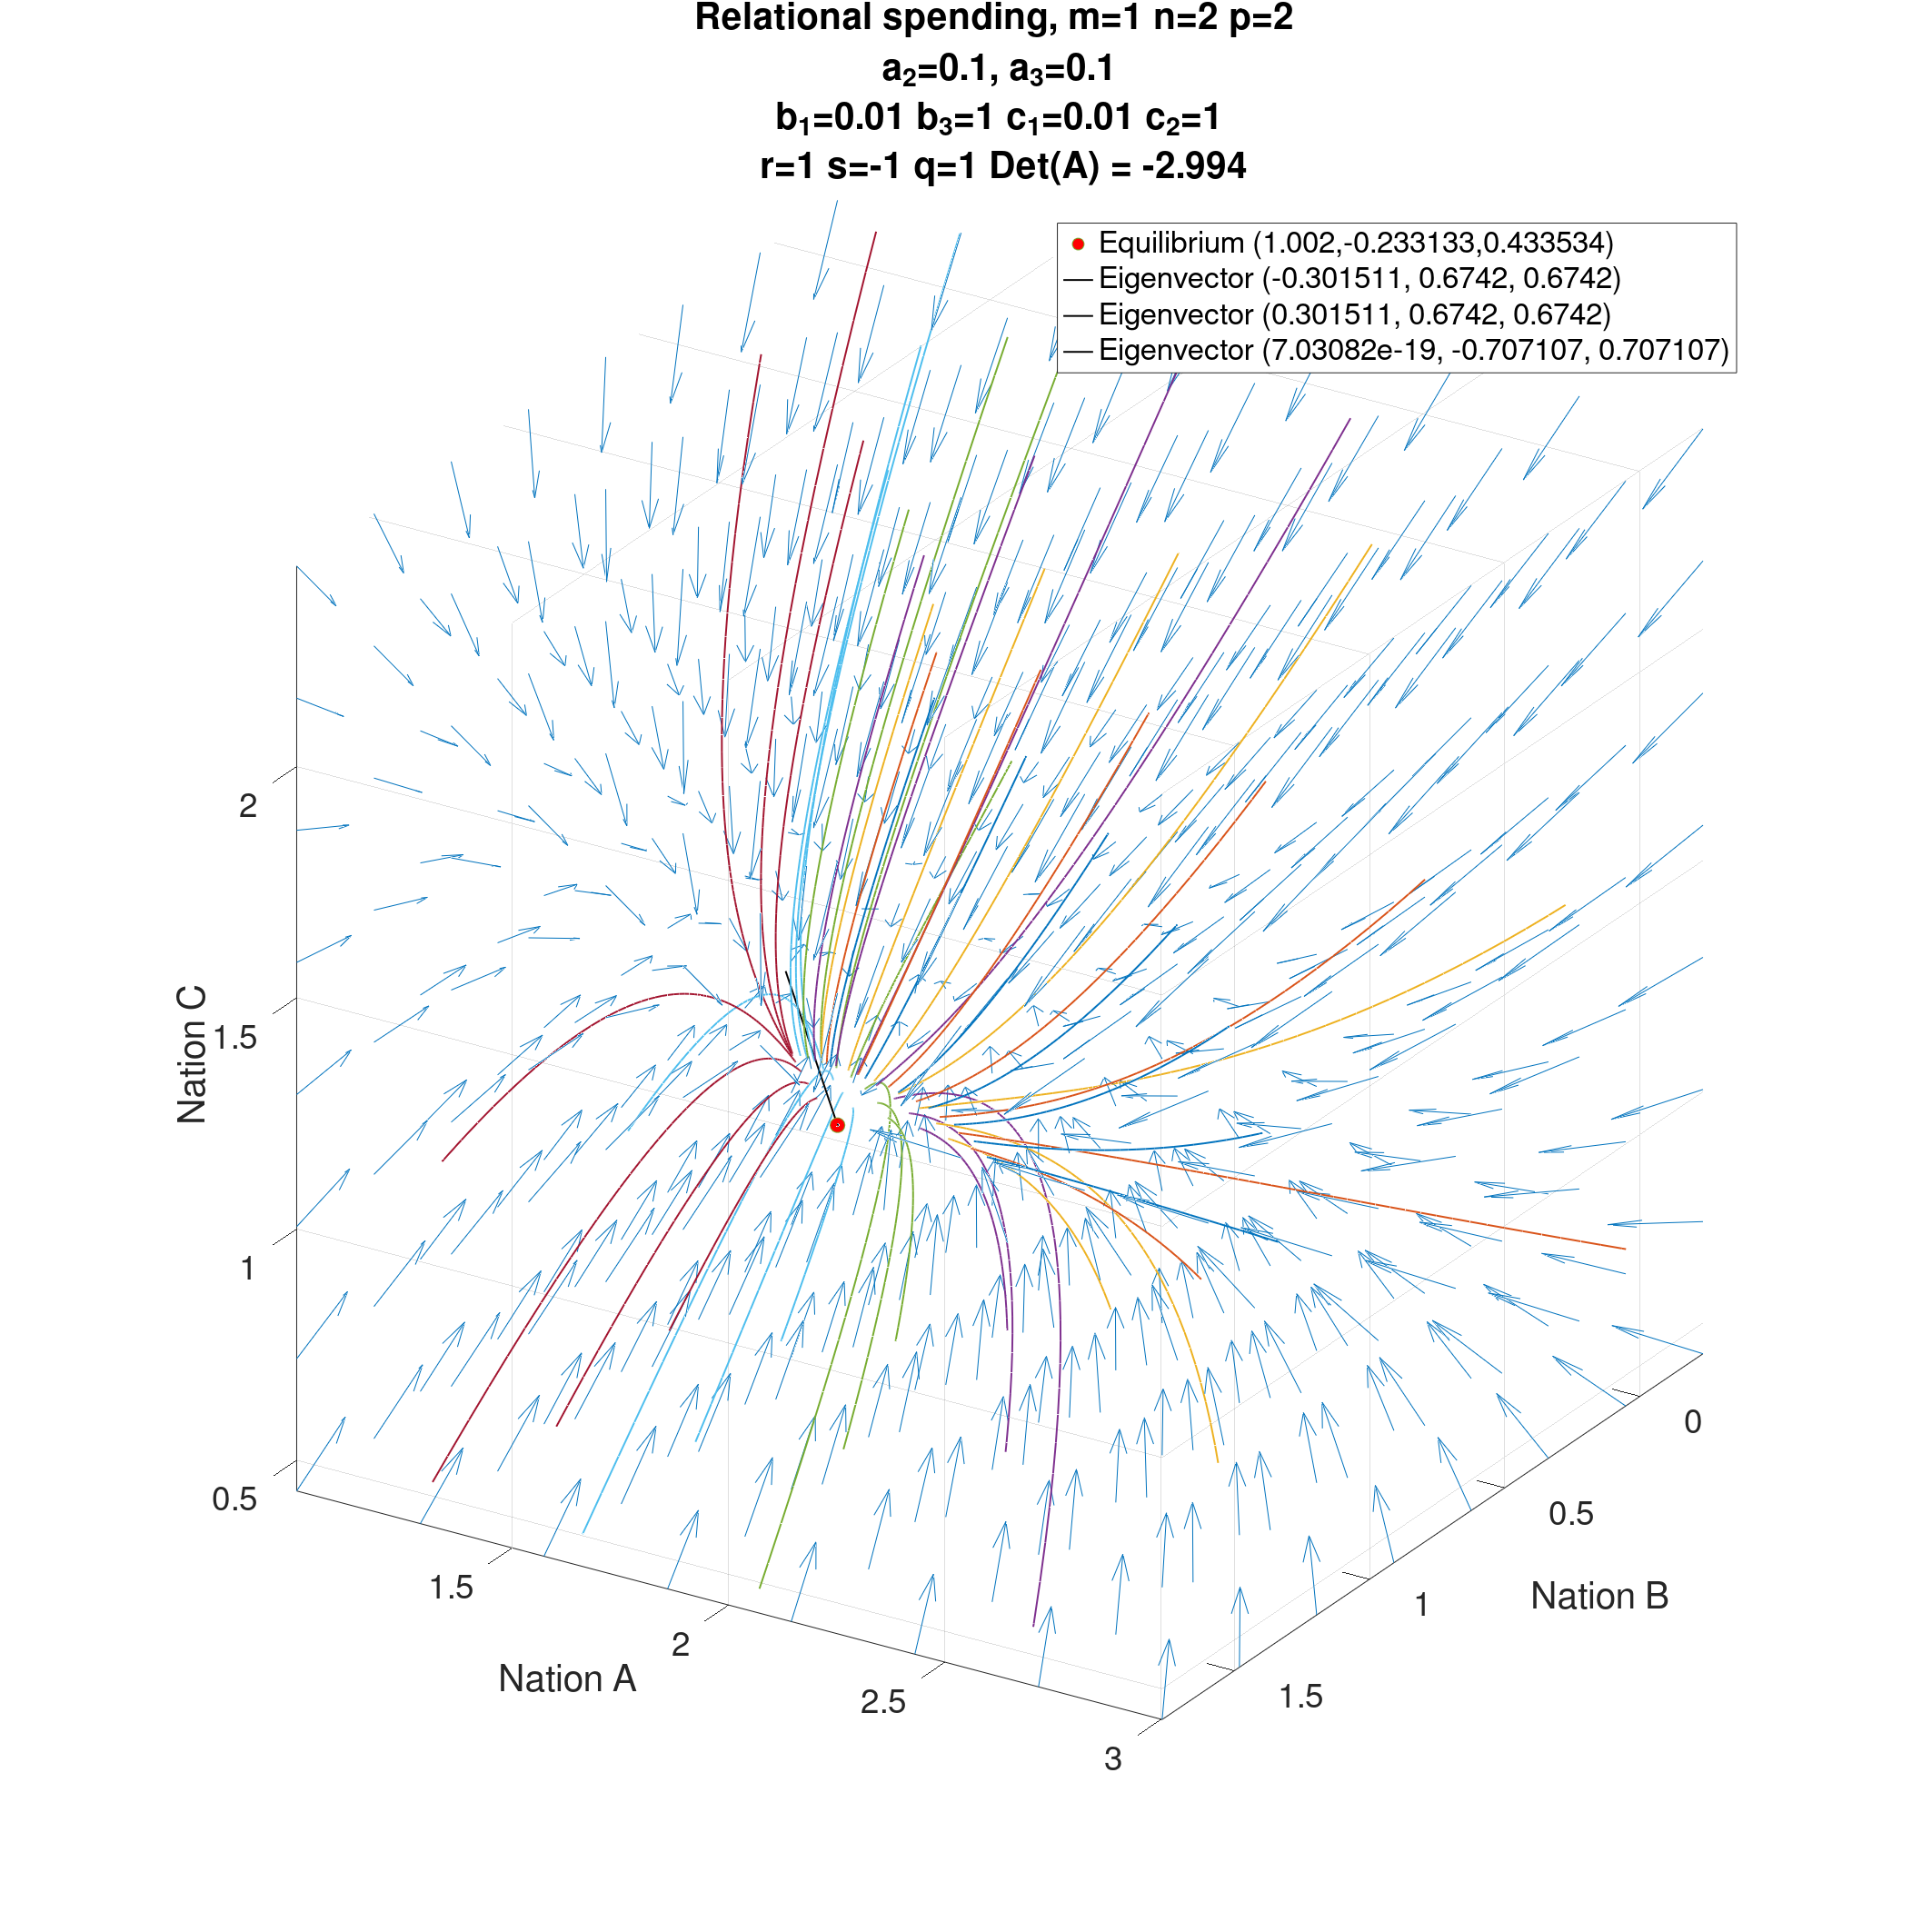
\includegraphics[height=0.9\textheight,width=\textwidth,keepaspectratio]{../figures/richardson_3D_1_-1_1.png}
    \end{figure}
\end{frame}
\begin{frame}{Future Goals}
  \begin{itemize}
    \item Streamline the codebase for less plugging in of parameters to generate the plots
    \item Transform into hyperbolic coordinates
      \begin{equation*}
	\left[u,v\right]^T=\left[A\cosh(\sqrt{ab}t+\phi),A\sinh(\sqrt{ab}t+\phi)\right]^T
      \end{equation*}
  to study the phase angle $\phi$ of the solution, and to extend the phase angle to the 3D case.
  \begin{itemize}
    \item \textbf{Idea: } the idea behind this is to compress the information about the parameters into a single value $\phi$ and to use it in conjunction with $\det{A}$ for a deeper understanding of Richardson's system.
  \end{itemize}
\item Study Richardson's work to further understand his point of view on arm's race modelling.
\end{itemize}
\end{frame}

\begin{frame}{References}
  \printbibliography
\end{frame}
\end{document}
